\section{Results}
To test the complete algorithm, several different scenarios have been used. Each scenario has unique characteristics and was tested with two different problem sizes. Theta* is always executed with a grid size of 2m and each time step has a duration of 200ms. All tests were executed on an Intel Core i5-4690k running at 4.4GHz with 16GB of 1600MHz DDR3 memory. The reported times are averages of 5 runs. The machine runs on Windows 10 using version 12.6 of IBM CPLEX. Figure \ref{fig:scenarios} shows these scenarios visually. Table \ref{table:results} shows detailed information about the scenarios and execution times.

\subsection{Up/Down Scenario}
The first test scenario has very few obstacles, but lays them out in a way such that the vehicle needs to slalom around them. The small scenario has only 5 obstacles, while the larger one has 9. This is a very challenging scenario for MILP because every obstacle has a large impact on the path. Without segmentation on the version of the scenario, the solver does not find the optimal path within 30 minutes. If execution is limited to 10 minutes, the best solution it finds takes 26.0s to execute by the vehicle. That is less than a second faster than the segmented result while it took more than 20 times more execution time to find that solution. For the larger scenario with 9 obstacles, the solver could not find a solution within 30 minutes. This scenario clearly shows the advantages of segmentation, even if there only are a few obstacles.

\subsection{San Francisco Scenario}
The San Francisco scenario covers a 1km by 1km section of the city for the small scenario, and 3km by 3km section for the large scenario. All the obstacles in this scenario are grid-aligned rectangles laid out in typical city blocks. Because of this, density of obstacles is predictable. This scenario showcases that the algorithm can scale to realistic scenarios with much more obstacles than is typically possible with a MIP approach. With these constraints, parameters and hardware, the path can be planned faster than the vehicle can execute it.

\subsection{Leuven Scenario}
The Leuven scenario also covers both a 1km by 1km and 3km by 3km section, this time of the Belgian city of Leuven. This is an old city with a very irregular layout. The dataset, provided by the local government\footnote{\url{https://overheid.vlaanderen.be/producten-diensten/basiskaart-vlaanderen-grb}}, also contains full polygons instead of the grid-aligned rectangles of the San Francisco dataset. While most buildings in the city are low enough so a UAV could fly over, it presents a very difficult test case for the path planning algorithm. The density of obstacles varies greatly and is much higher than in the San Francisco dataset across the board. The algorithm does slow down, but it is still fast enough for offline planning. As visible in figure \ref{fig:pre-3-4}, there are many obstacles clustered close to each other, with many edges being completely redundant. For a real application, a small amount of preprocessing of the map data should be able to significantly reduce both the amount of obstacles as the amount of edges. 

\begin{figure}
	\centering
	\subfloat{
        	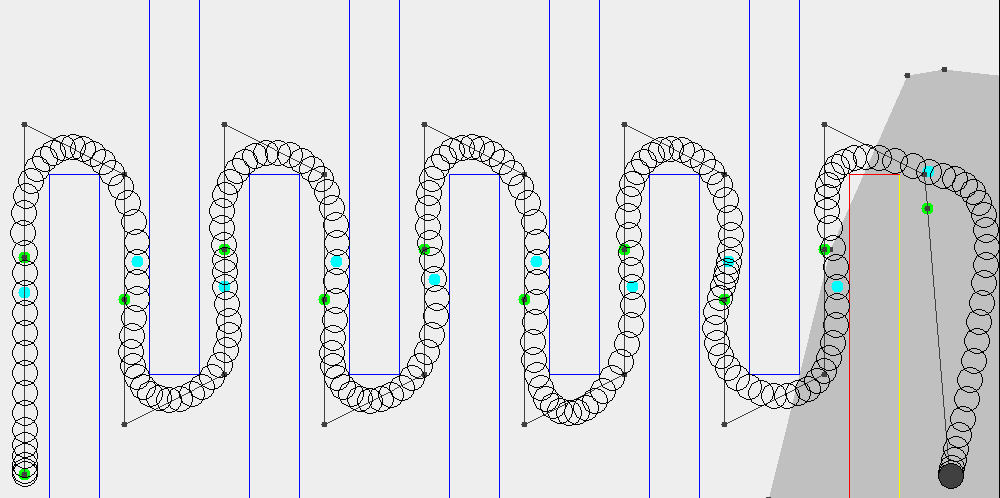
\includegraphics[width=0.7\columnwidth]{img/benchmarkfull}
	}

          \subfloat{
        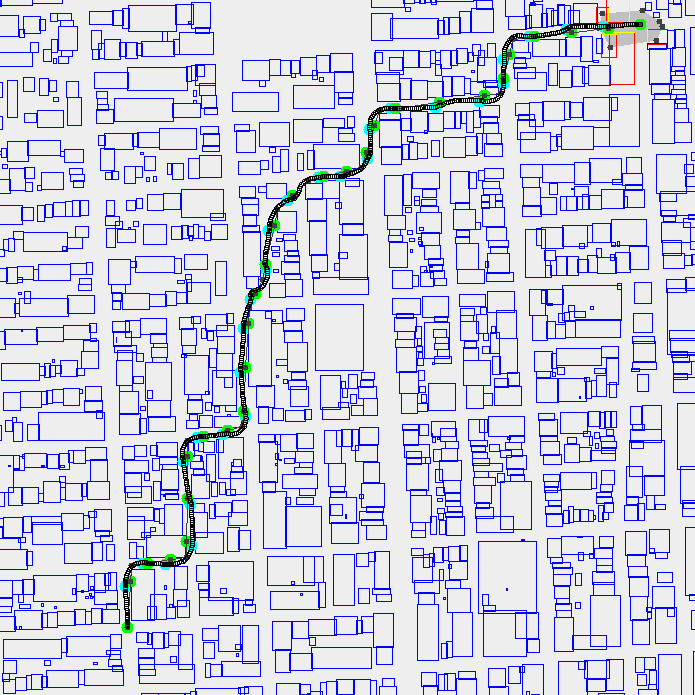
\includegraphics[width=0.7\columnwidth]{img/SF}
	}

          \subfloat{
        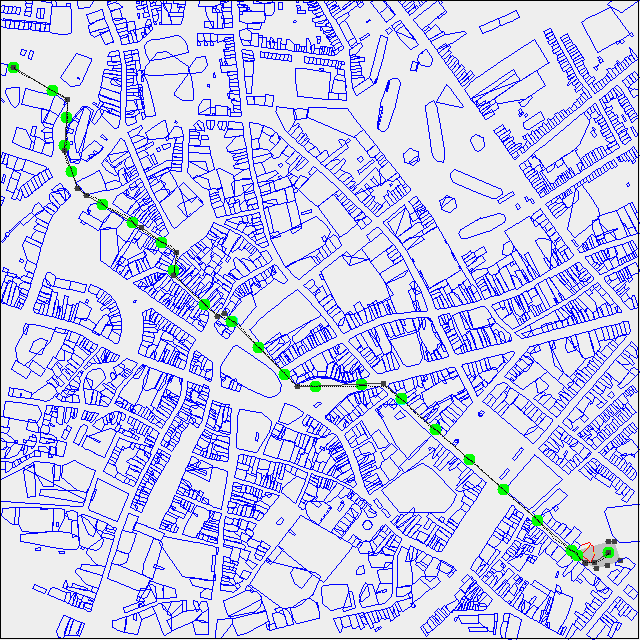
\includegraphics[width=0.7\columnwidth]{img/leuven}
        }
        
    \caption{These are the three different worlds which were tested. The top image shows the large up/down scenario. The middle image shows the small San Fransisco scenario. Note how the obstacles are only grid-aligned rectangles laid out in a grid pattern. The bottom image shows the small Leuven scenario. The obstacles are polygons and distributed in a much more irregular pattern compared to the San Fransisco scenario.}\label{fig:scenarios}
\end{figure}


\begin{figure*}
\begin{tabular}{ c c c c c c c c c }
 scenario & obstacles & world size & path length & segments & Theta* time & GA time & MILP time & score \\ 
up/down small & 5 &  25m x 20m & 88m  & 7 & 0.09s & 1.10s & 20.8s & 26.6s\\
up/down large & 9 & 40m x 20m &  146m & 11 & 0.14s & 1.62s & 40.1s & 43.6s \\
SF small & 684 & 1km x 1km & 1392m & 28 & 2.04s & 9.56s & 59.2s & 106s \\
SF large & 6580 & 3km x 3km & 4325m  & 84 & 18.14s & 18.21 & 231s & 316s\\
Leuven small & 3079 & 1km x 1km & 1312m & 29 &  2.29s & 29.83s & 152s  & 96s \\
Leuven large & 18876 & 3km x 3km & 3041m & 61 & 18.14 & 83.69s & 687s & 218s \\

\end{tabular}
\caption{Some relevant data about the different scenarios}
\label{table:results}
\end{figure*}

\section{Conclusion}
Path planning using MIP was previously not computationally possible in large and complex environments. The approach presented in this paper shows that these limitations can effectively be circumvented by dividing the path into smaller segments using several steps of preprocessing. The specific algorithms used in each step to generate the segments can be swapped out easily with variations. Because the final path is generated by a solver, the constraints on the path can also be easily changed to account for different use cases. The experimental results show that the algorithm works well in realistic, city-scale scenarios, even when obstacles are distributed irregularly and dense.

\subsection{Future Work}
The results so far are promising, but have not been used on real hardware yet. Extending the software we built so it can be tested with actual hardware is an obvious next step. That also leads to the next possible extension: Currently the algorithm works in 2D, but extending it to 3D would allow it to be used in more kinds of environments. We'd also like to allow for more kinds of constraints on the path of the vehicle.